\documentclass[9pt,aspectratio=169]{beamer}
\mode<presentation>
\usepackage[T1]{fontenc}
\usepackage{color}
\usepackage{graphicx}
\usepackage{natbib}
\usepackage{listings}

\definecolor{codegreen}{rgb}{0,0.6,0}
\definecolor{codegray}{rgb}{0.5,0.5,0.5}
\definecolor{codepurple}{rgb}{0.58,0,0.82}
\definecolor{backcolour}{rgb}{0.95,0.95,0.92}

\lstdefinestyle{mystyle}{
	backgroundcolor=\color{backcolour},   
	commentstyle=\color{codegreen},
	keywordstyle=\color{magenta},
	numberstyle=\tiny\color{codegray},
	stringstyle=\color{codepurple},
	basicstyle=\ttfamily\footnotesize,
	breakatwhitespace=false,         
	breaklines=true,                 
	captionpos=b,                    
	keepspaces=true,                 
	numbers=left,                    
	numbersep=5pt,                  
	showspaces=false,                
	showstringspaces=false,
	showtabs=false,                  
	tabsize=2
}

\lstset{style=mystyle}

\usepackage{hyperref}

\usetheme{Singapore}
%\usecolortheme{seahorse}

\usefonttheme{professionalfonts}

\title[LLM screening and coding]{Screening and coding with LLMs}

\author{Max Callaghan}
\institute[MCC]{

\includegraphics[height=1cm,width=2cm]{images/MCC_Logo_RZ_rgb.jpg}
}



\newtheorem*{remark}{}

\bibliographystyle{apalike}

\begin{document}

\begin{frame}
\titlepage
\end{frame}

\begin{frame}{Outlook}
	\begin{itemize}
		\item<1-> Results from the implementation of \cite{wang_zero-shot_2024}
		\item<2-> Additional results from Santiago's thesis project on coding
	\end{itemize}
\end{frame}

%\section{Introduction}
%
%\section{Implementation}

\section{Screening}

\begin{frame}{We can ask LLMs whether a study should be included in a systematic review}
	\begin{columns}
		\begin{column}{0.5\linewidth}
			\begin{figure}
				\footnotesize
				%\includegraphics[width=\linewidth]{images/example.txt}
				\input{images/example.txt}
			\end{figure}
		\end{column}
		\begin{column}{0.5\linewidth}
			\only<2->{\begin{figure}
					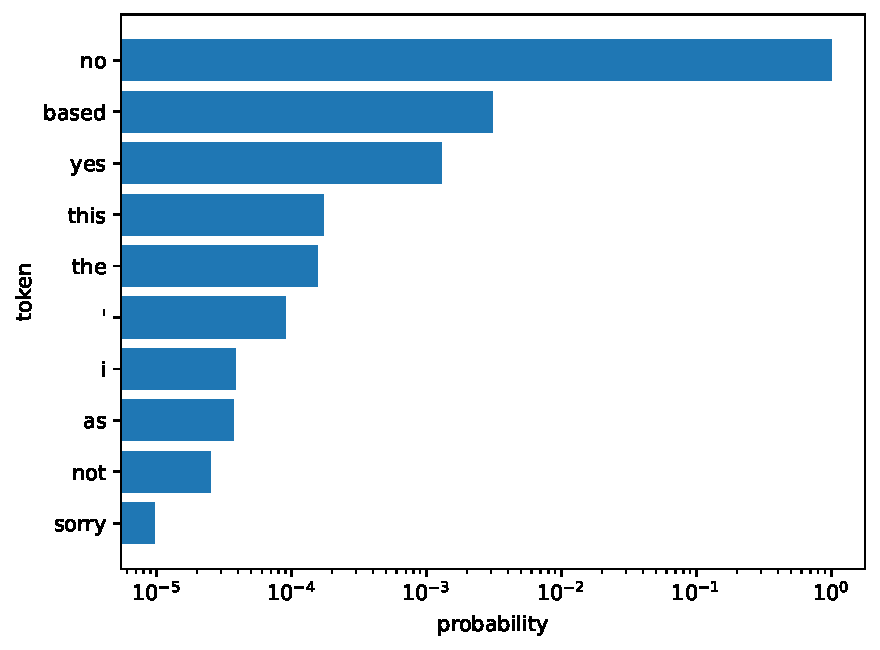
\includegraphics[width=\columnwidth]{images/example_probs.pdf}
			\end{figure}}
		\end{column}
	\end{columns}
\end{frame}

\begin{frame}{Zero-shot Generative Large Language Models for Systematic Review Screening Automation}
	
	\cite{wang_zero-shot_2024} propose a method to extract probability-like scores from LLMs for inclusion/exclusion decisions in a systematic review
	
	\begin{figure}
		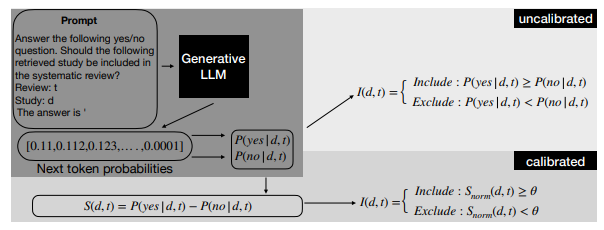
\includegraphics[width=\columnwidth]{images/fig1}
	\end{figure}
\end{frame}

\begin{frame}{Results are mixed, because the probabilities are poorly calibrated, and their attempts to re-invent stopping criteria do not makes sense}
	
	
	
	\begin{figure}
		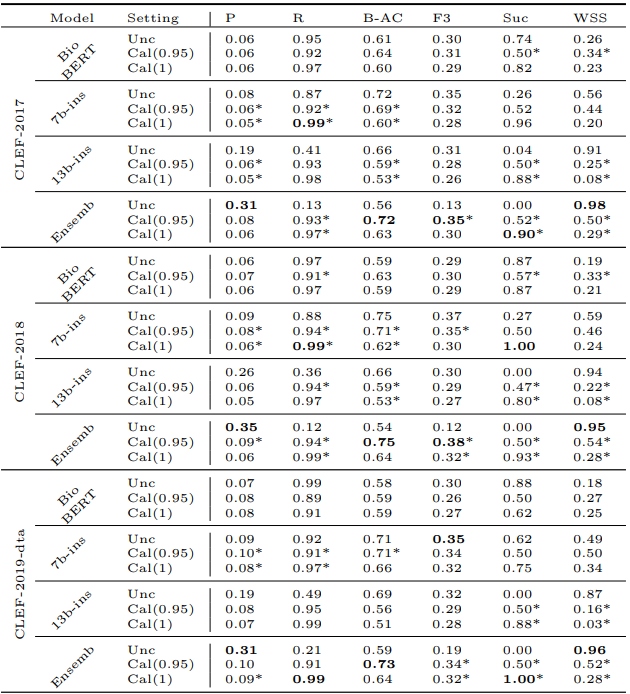
\includegraphics[width=0.8\columnwidth]{images/tab3-1}
	\end{figure}
\end{frame}



\begin{frame}[fragile]{Implementation is relatively straightforward}
\small
\begin{lstlisting}[language=Python]
def binary_probs(tokenizer, model, prompt, no_words=['no'], yes_words=['yes'], return_all=False):
    device = 'cuda' if torch.cuda.is_available() else 'cpu'
    encoded_text = tokenizer(prompt, return_tensors="pt").to(device)
    #1. step to get the logits of the next token
    with torch.inference_mode():
        outputs = model(**encoded_text)

    next_token_logits = outputs.logits[0, -1, :]

    # 2. step to convert the logits to probabilities
    next_token_probs = torch.softmax(next_token_logits, -1)

    topk_next_tokens= torch.topk(next_token_probs, 50)
    tokens = [tokenizer.decode(x).strip().lower() for x in topk_next_tokens.indices]
    p = topk_next_tokens.values

    df = pd.DataFrame.from_dict({'t': tokens,'p': p.cpu()})
    y = df[df['t'].isin(yes_words)]['p'].sum()
    n = df[df['t'].isin(no_words)]['p'].sum()

    if return_all:
        return df.groupby('t').sum().reset_index().sort_values('p', ascending=False).reset_index(drop=True)
    return y-n, y+n
\end{lstlisting}

\end{frame}

\begin{frame}[fragile]{Implementation is relatively straightforward}
	\small
\begin{lstlisting}[language=Python]
prompt = Template('''<s>[INST] <<SYS>>
You are a systematic review helper tasked with finding out whether a study is relevant to the review $t

Answer 'yes' if the study is relevant, or 'no' if not
<</SYS>>

Study: $s 

Should the study be included? Answer yes or no. [/INST] ''')

prompt.substitute({'t': review, 's': study_title}),
\end{lstlisting}
	
\end{frame}

%\section{Results}

\begin{frame}{Result \#1: It works!}
	\begin{columns}
		\begin{column}{0.4\linewidth}
			\begin{itemize}
				\item<1-> The method produces a ranking that identifies all relevant documents before all documents have been screened
				\item<2-> But it doesn't perform as well as simple tfidf + SVM
				\item<3-> To compare the quality of rankings, we can use ROC AUC scores
			\end{itemize}
		\end{column}
		\begin{column}{0.6\linewidth}
			\only<1>{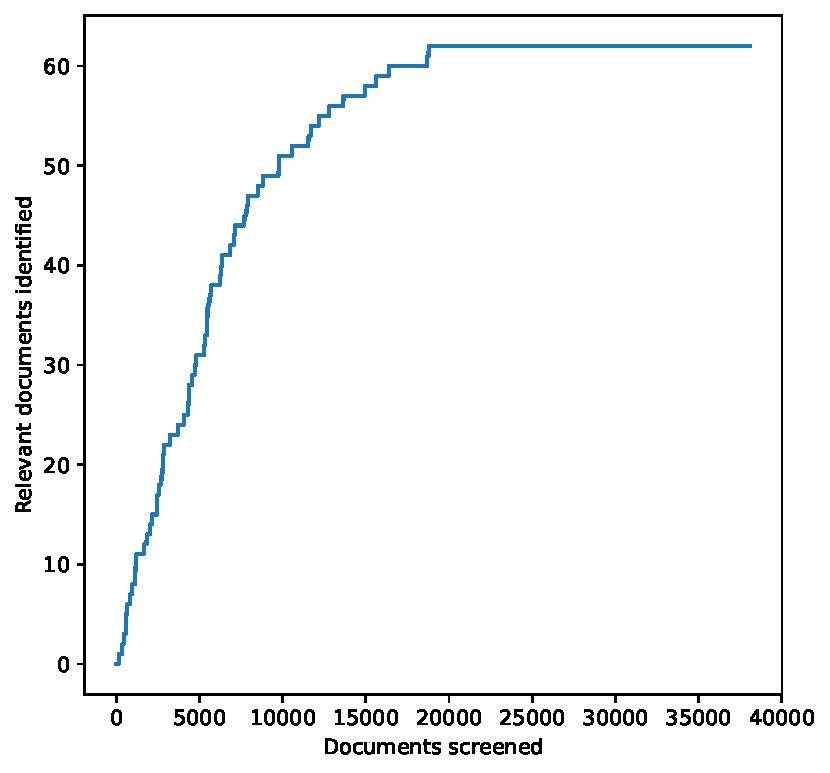
\includegraphics[width=\linewidth]{../../figures/LLM_Brouwer_simple.pdf}}
			\only<2->{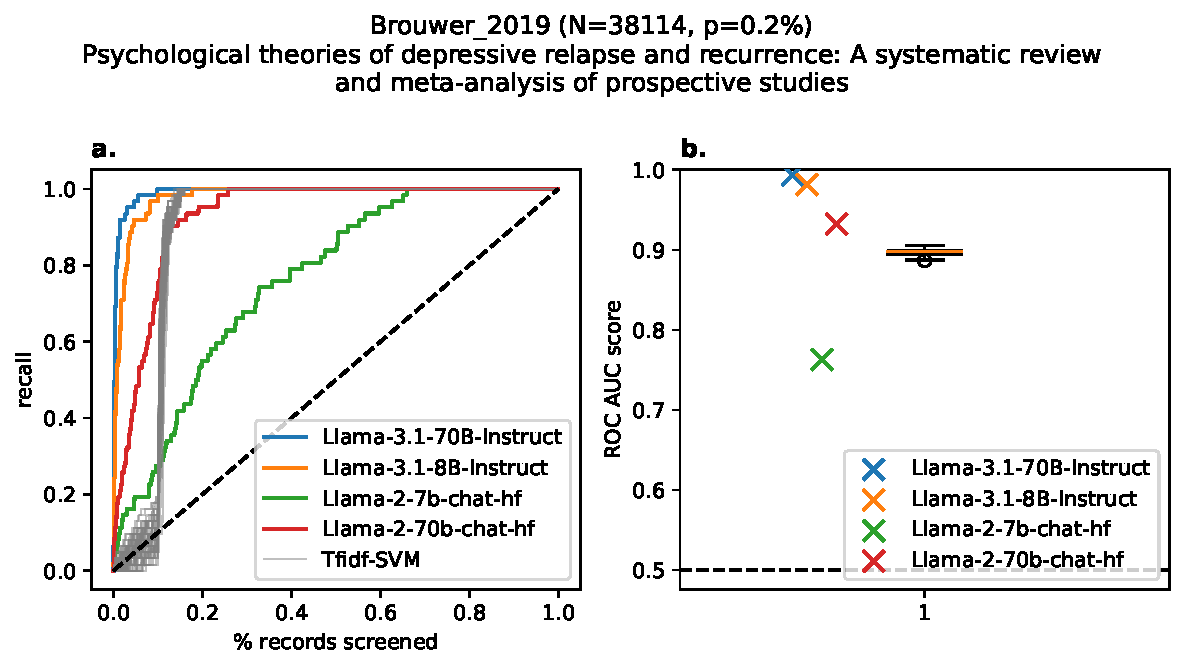
\includegraphics[width=\linewidth]{../../figures/Brouwer_2019.pdf}}
			%\only<3>{}
		\end{column}
	\end{columns}
\end{frame}



\begin{frame}{This method simply produces a ranking of documents, but is this ranking better than what we can produce with traditional active learning approaches?}
	
	\begin{columns}
		\begin{column}{0.618\linewidth}
			\begin{figure}
				
				\only<1>{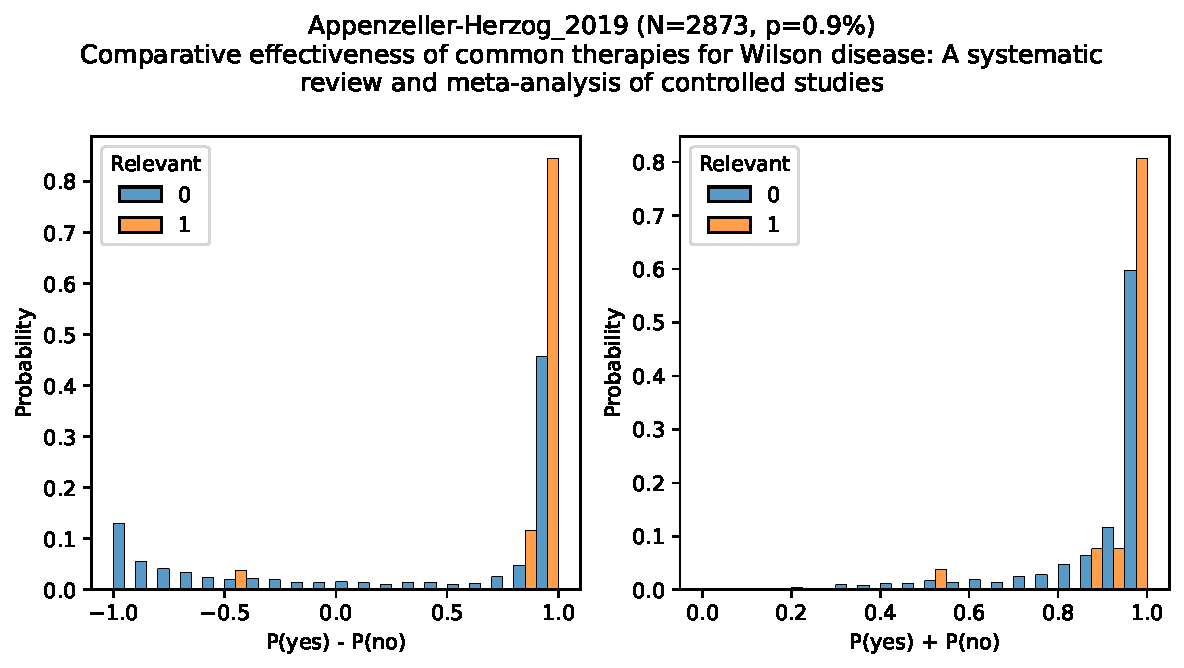
\includegraphics[width=\columnwidth]{../../figures/Appenzeller-Herzog_2019_p_distribution.pdf}}
				\only<2>{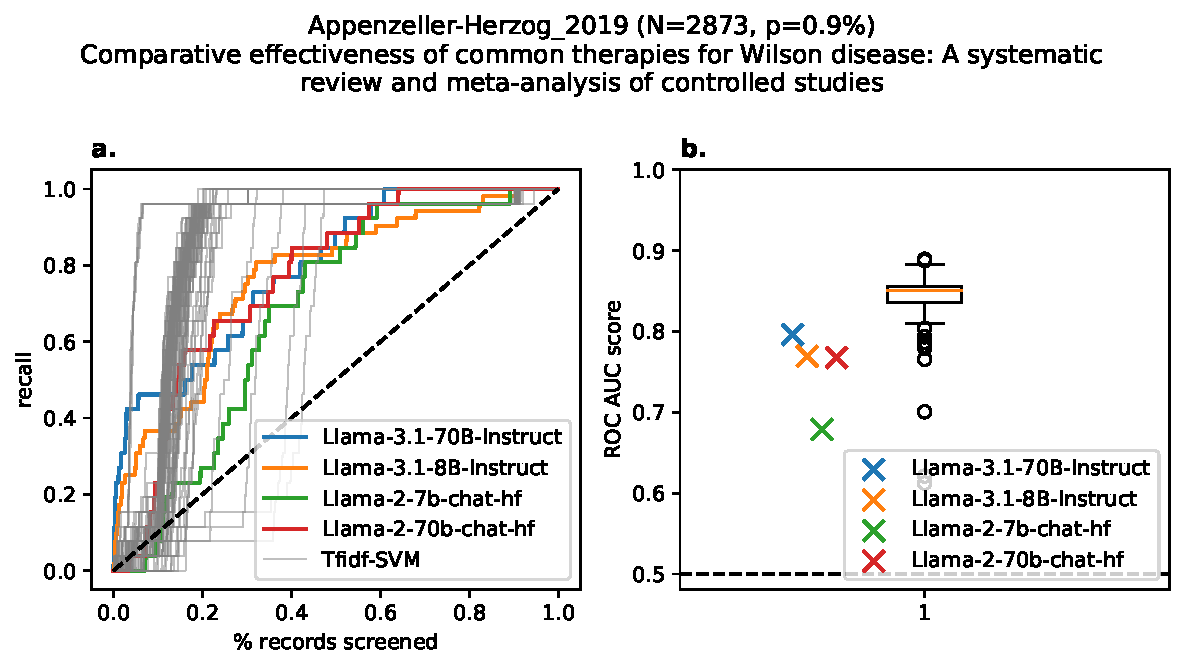
\includegraphics[width=\columnwidth]{../../figures/Appenzeller-Herzog_2019.pdf}}
				\only<3>{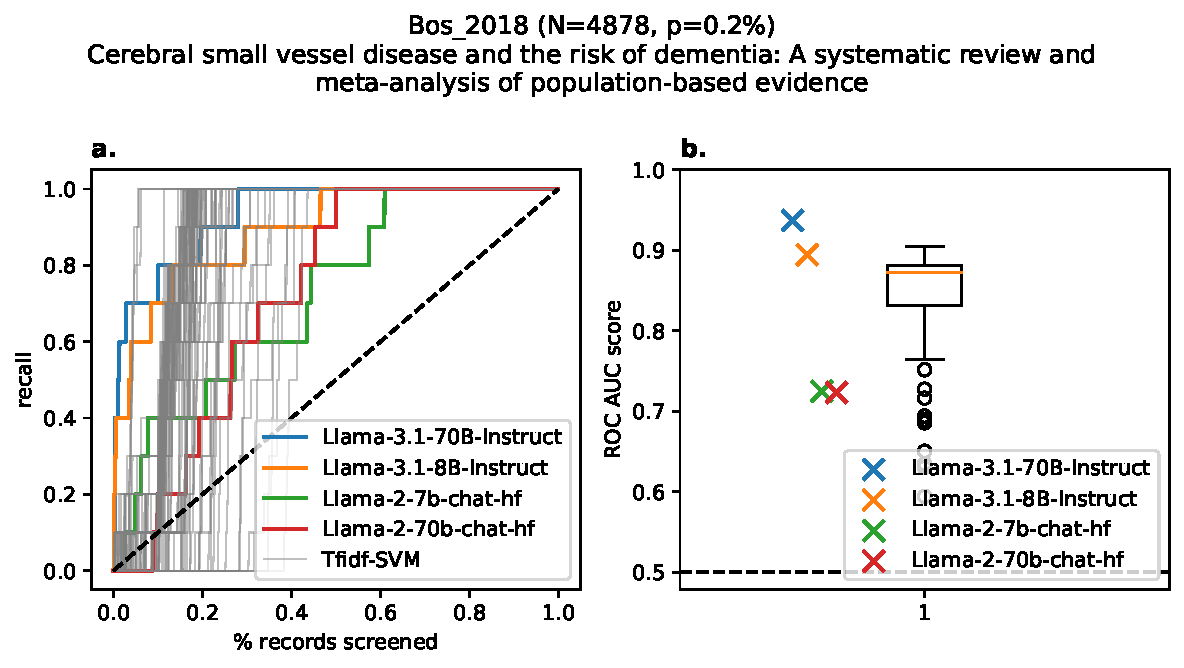
\includegraphics[width=\columnwidth]{../../figures/Bos_2018.pdf}}
				\only<4>{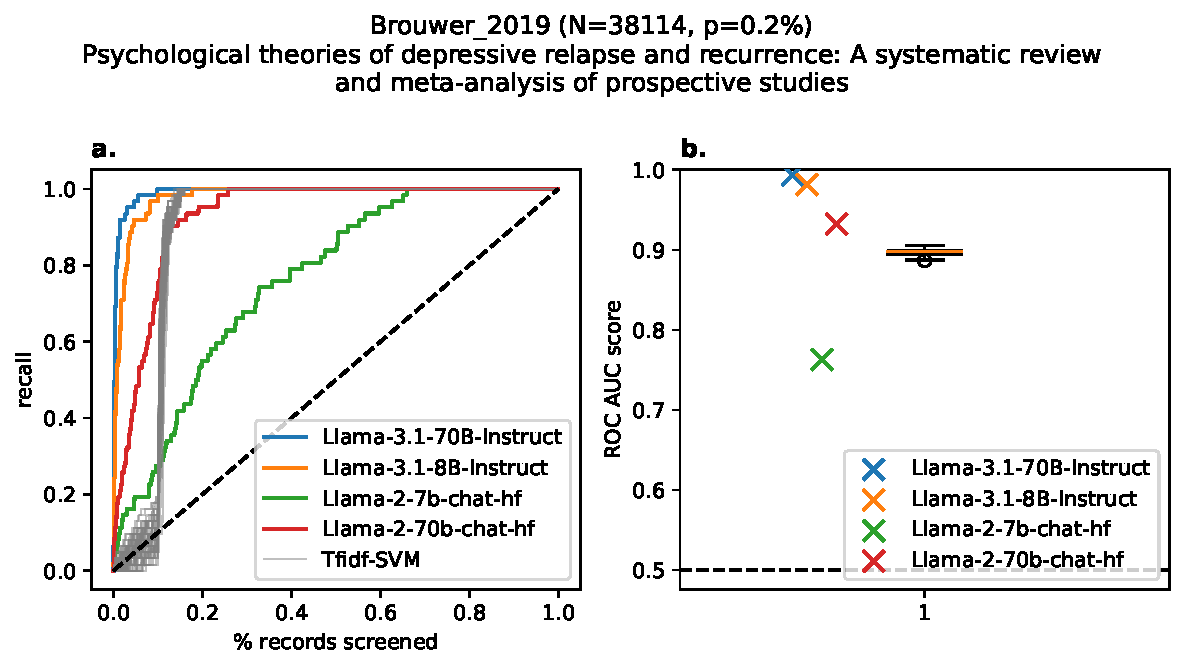
\includegraphics[width=\columnwidth]{../../figures/Brouwer_2019.pdf}}
				\only<5>{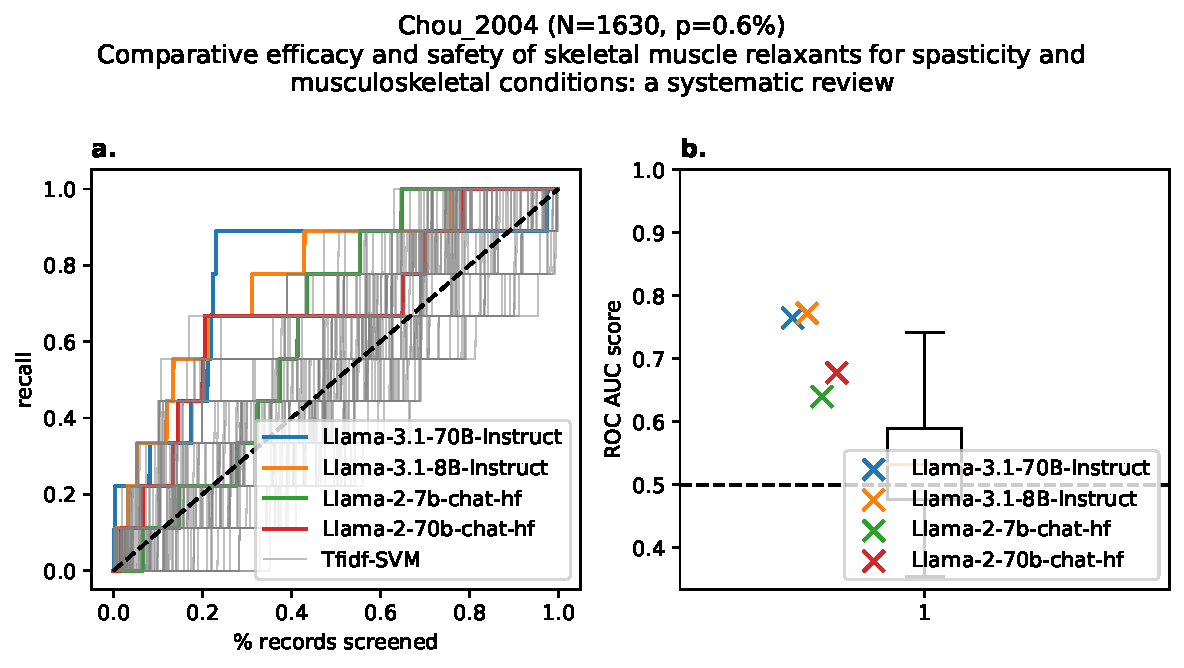
\includegraphics[width=\columnwidth]{../../figures/Chou_2004.pdf}}
				\only<6>{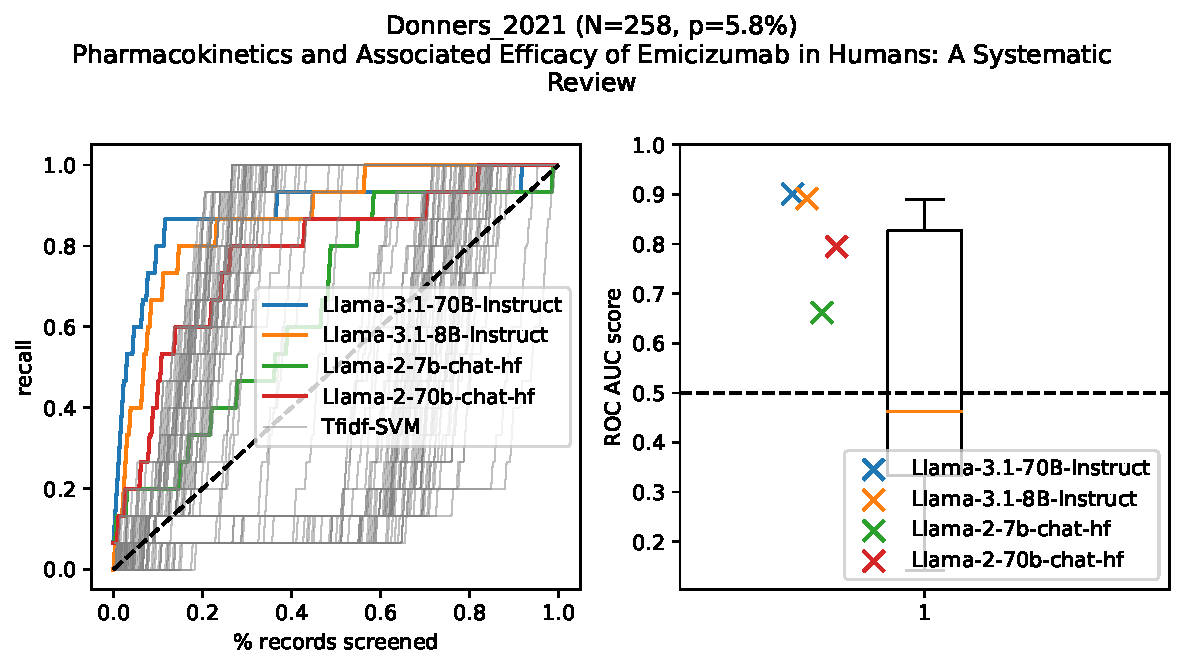
\includegraphics[width=\columnwidth]{../../figures/Donners_2021.pdf}}
				\only<7>{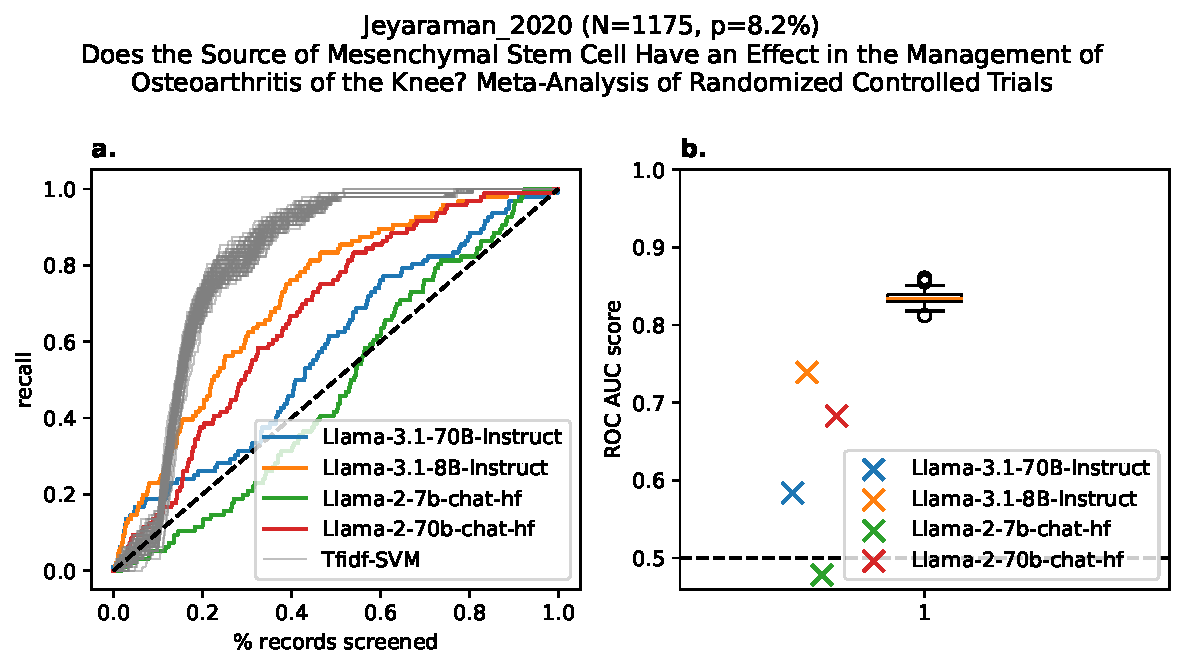
\includegraphics[width=\columnwidth]{../../figures/Jeyaraman_2020.pdf}}
			\end{figure}
		\end{column}
		\begin{column}{0.382\linewidth}
			\begin{itemize}
				\item<1-> We generated LLM inclusion scores for each document in a set of reviews in the Synergy dataset
				\item<2-> We compare what happens to screening in descending order of this ranking to 100 active learning runs with a default configuration of SVM with Tfidf
				\item<3-> Initial results are not very promising
				\item<5->But LLMs can do well where traditional methods struggle
				\item<7->Sometimes they are no use at all
			\end{itemize}
		\end{column}
	\end{columns}
	
	
	

\end{frame}

\begin{frame}{All results}
	\begin{columns}
	\begin{column}{0.618\linewidth}
		\begin{figure}
			
			\only<1->{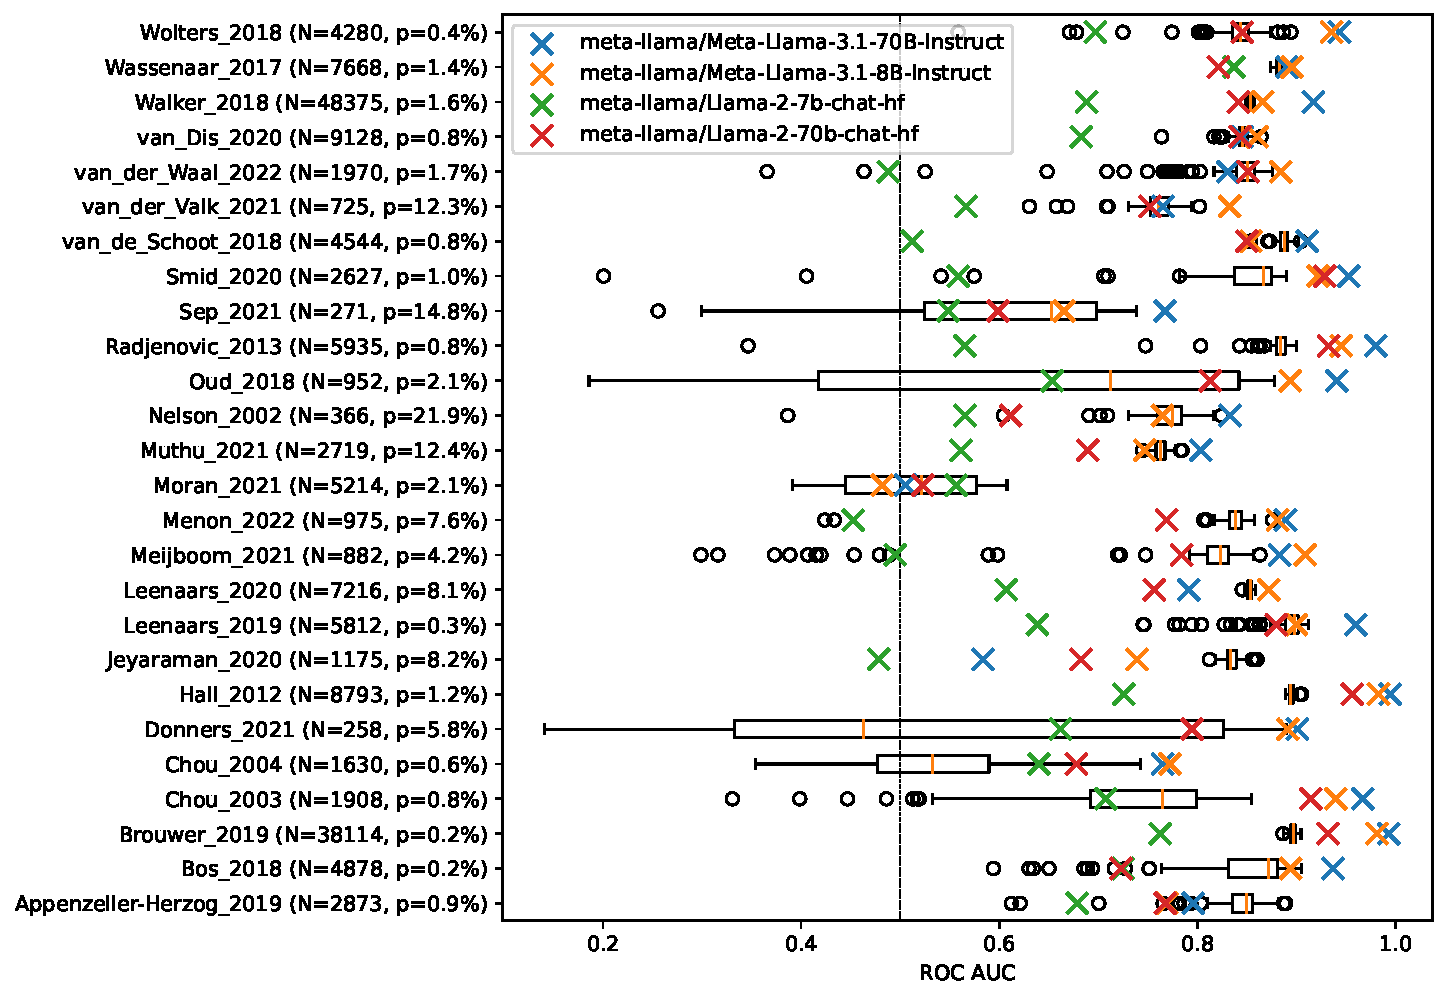
\includegraphics[width=\columnwidth]{../../figures/llm_svm_roc.pdf}}

		\end{figure}
	\end{column}
	\begin{column}{0.382\linewidth}
		\begin{itemize}
			\item<1-> LLMs and basic active learning pipelines seem to have different weakneses
			\item<2-> Combining both could improve general performance
			\item<3-> LLMs seem most useful for smaller datasets (where active learning has little time to learn)
		\end{itemize}
	\end{column}
\end{columns}
\end{frame}

%\section{Conclusion}

\begin{frame}{Some things still to explore}
	
\begin{itemize}
	\item<1-> Prompting strategies (inclusion criteria)
	\item<2-> Bigger/different models
	\item<3-> Combining LLMs with traditional approaches
	\item<4-> Updating prompts based on user feedback
\end{itemize}

\end{frame}

\begin{frame}{Conclusions}
	\begin{columns}
		\begin{column}{0.4\linewidth}
			\begin{itemize}
				\item<1-> LLMs are neither a quick fix or a silver bullet
				\item<2-> Evaluation is vital
				\item<3-> We can't forget the need for appropriate stopping criteria \cite{callaghan_statistical_2020}
				%\item<4->\url{mcallaghan.github.io/buscar-app}
			\end{itemize}
		\end{column}
		\begin{column}{0.6\linewidth}
			\begin{figure}
				\only<3>{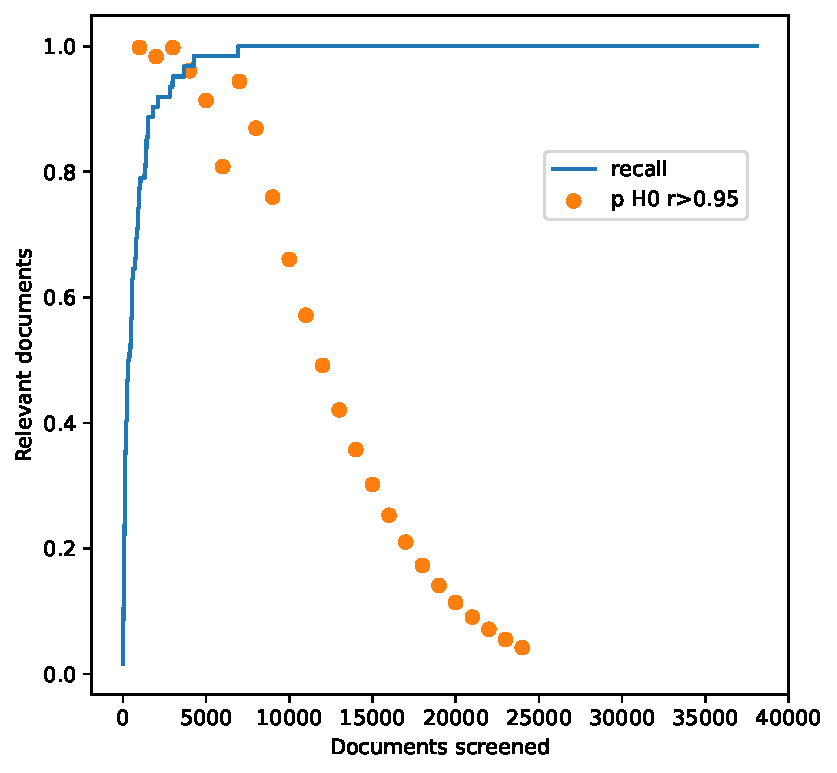
\includegraphics[width=\columnwidth]{../../figures/stopping.pdf}}
			\end{figure}
		\end{column}
	\end{columns}

\end{frame}

\section{Coding}
	
\begin{frame}{Using LLMs for coding}
		\begin{columns}
		\begin{column}{0.4\linewidth}
			\begin{itemize}
				\item<1-> Santiago's thesis showed us that LLMs can achieve comparable performance with BERT-type models
				\item<2->They need no training data to achieve this performance
				\item<3->But we do need annotated data for ``prompt engineering'' ($\approx$ training?), and for evaluation
			\end{itemize}
		\end{column}
		\begin{column}{0.6\linewidth}
			\begin{figure}
				\only<1->{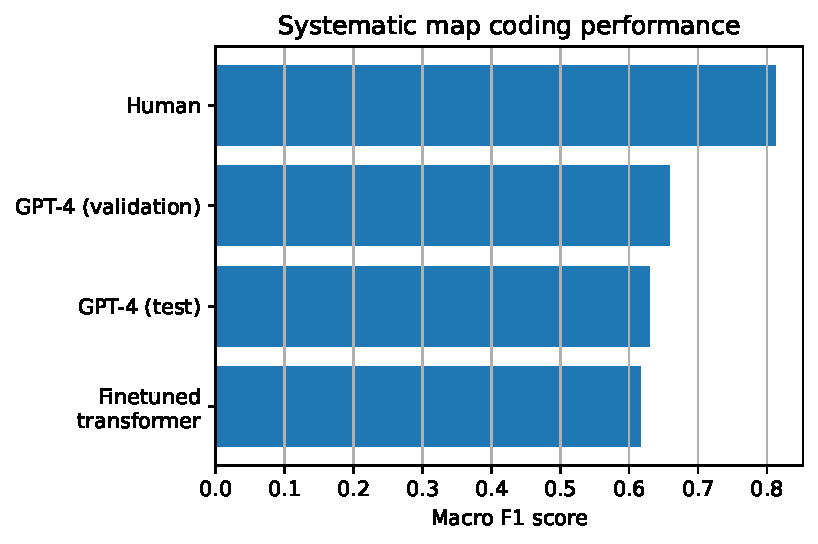
\includegraphics[width=\columnwidth]{../../figures/LLM-coding.pdf}}
			\end{figure}
		\end{column}
	\end{columns}
	
\end{frame}

\begin{frame}{Using LLMs for coding}
	\begin{columns}
		\begin{column}{0.4\linewidth}
			\begin{itemize}
				\item<1-> Results were aggregated Macro F1 scores for 30 labels
				\item<2-> Aggregate results hide much variation
				\item<3-> This varies across the different coding categories
				\item<4-> And there seems to be a clear correlation with number of labels
			\end{itemize}
		\end{column}
		\begin{column}{0.6\linewidth}
			\begin{figure}
				\only<2>{\includegraphics[width=\columnwidth]{../../../LLM-eval/gpt/figures/BERT-vs-LLMs.pdf}}
				\only<3>{\includegraphics[width=\columnwidth]{../../../LLM-eval/gpt/figures/BERT-vs-LLMs-categories.pdf}}
				\only<4>{\includegraphics[width=\columnwidth]{../../../LLM-eval/gpt/figures/BERT-vs-LLMs-n.pdf}}
			\end{figure}
		\end{column}
	\end{columns}


	
\end{frame}

	\begin{frame}{Conclusions}
\end{frame}
%	
%\begin{frame}
%	Thanks!
%	
%	\bigskip
%	
%	\hrule
%	
%	\bigskip
%	
%	\url{callaghan@mcc-berlin.net}
%	 
%	\medskip
%	
%	Twitter: @MaxCallaghan5
%	
%	\bigskip
%	
%	\begin{figure}
%	
\includegraphics[width=0.1\columnwidth]{images/wellcome-logo-black.eps}
%	\end{figure}
%\end{frame}
%	



\begin{frame}
	\bibliography{../LLMs}
\end{frame}

\end{document}